\documentclass[tikz,border=8pt]{standalone}
\usepackage{amsmath}
\usetikzlibrary{arrows.meta}
\definecolor{ink}{HTML}{21352F}
\definecolor{teal}{HTML}{087F7B}
\definecolor{blue}{HTML}{4B77A8}
\definecolor{gold}{HTML}{C58B2A}
\definecolor{rose}{HTML}{B65A62}
\begin{document}
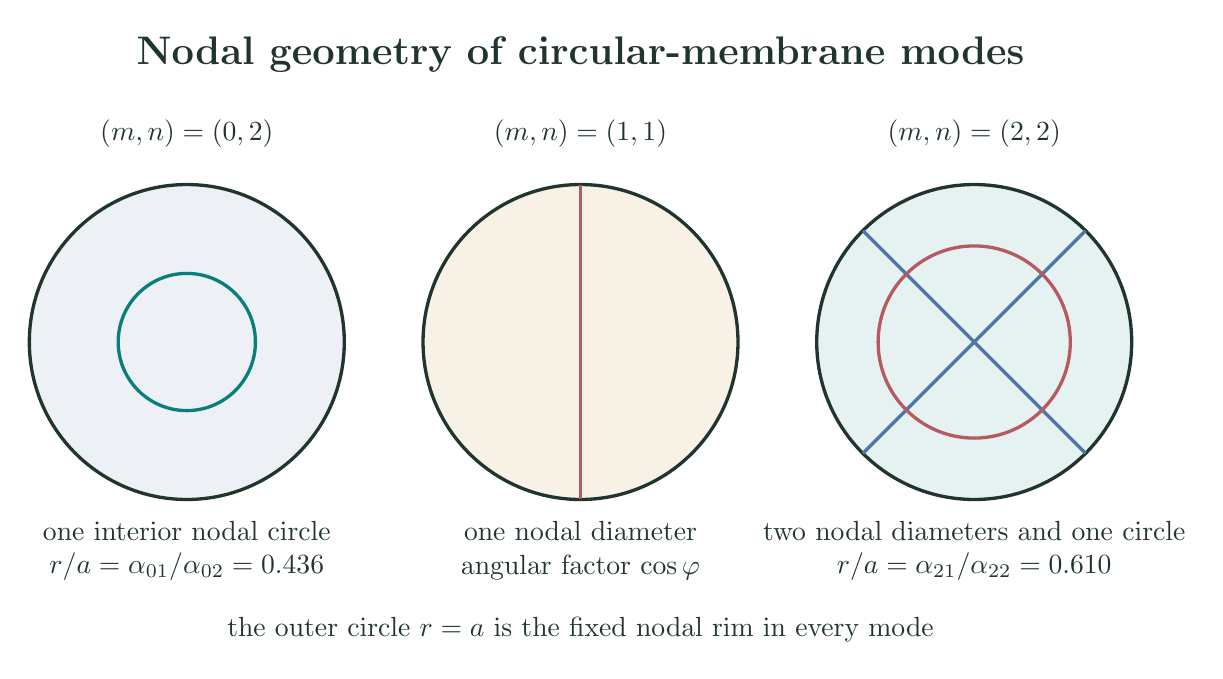
\begin{tikzpicture}[font=\large\sffamily,text=ink]
  \node[font=\bfseries\Large] at (0,3.65)
    {Nodal geometry of circular-membrane modes};

  \begin{scope}[xshift=-5cm]
    \fill[blue!10] (0,0) circle (2);
    \draw[ink,very thick] (0,0) circle (2);
    \draw[teal,very thick] (0,0) circle ({2*2.4048/5.5201});
    \node[font=\bfseries] at (0,2.65) {$(m,n)=(0,2)$};
    \node[align=center,font=\normalsize] at (0,-2.65)
      {one interior nodal circle\\
       $r/a=\alpha_{01}/\alpha_{02}=0.436$};
  \end{scope}

  \begin{scope}
    \fill[gold!12] (0,0) circle (2);
    \draw[ink,very thick] (0,0) circle (2);
    \draw[rose,very thick] (0,-2)--(0,2);
    \node[font=\bfseries] at (0,2.65) {$(m,n)=(1,1)$};
    \node[align=center,font=\normalsize] at (0,-2.65)
      {one nodal diameter\\
       angular factor $\cos\varphi$};
  \end{scope}

  \begin{scope}[xshift=5cm]
    \fill[teal!10] (0,0) circle (2);
    \draw[ink,very thick] (0,0) circle (2);
    \draw[blue,very thick] (-1.414,-1.414)--(1.414,1.414);
    \draw[blue,very thick] (-1.414,1.414)--(1.414,-1.414);
    \draw[rose,very thick] (0,0) circle ({2*5.1356/8.4172});
    \node[font=\bfseries] at (0,2.65) {$(m,n)=(2,2)$};
    \node[align=center,font=\normalsize] at (0,-2.65)
      {two nodal diameters and one circle\\
       $r/a=\alpha_{21}/\alpha_{22}=0.610$};
  \end{scope}

  \node[font=\normalsize] at (0,-3.65)
    {the outer circle $r=a$ is the fixed nodal rim in every mode};
\end{tikzpicture}
\end{document}
